\section{Funktionsweise des Chainwebs}
\label{sec:chainweb_overview}
Das Chainweb ist eine öffentlich zugängliche Blockchain. Diese setzt zur Konsensfindung auf das bewährte Proof of Work Verfahren. Die Überlegung ist es, eine POW-Blockchain auf Layer 1 zu skalieren. Das Chainweb besteht aus mehreren unabhängigen und parallelen Ketten. Auf jeder Kette wird ähnlich zu Bitcoin der native Coin KDA geschürft. Zusätzlich wird im Header neben dem vorherigen Block auch auf vorangegangene Blöcke der parallelen Ketten gezeigt. Alle 30 Sekunden wird auf jeder Kette ein neuer Block generiert.  Zur Veranschaulichung dient der in Abbildung \eqref{fig:petersen_graph_10} gezeichnete Petersen-Graph. Die Ordnung des Graphen spiegelt die Anzahl der Ketten wider, der Grad gibt Auskunft über die Anzahl der Kanten eines jeden Knoten und der Durchmesser beschreibt, in wie vielen Schritten maximal ein Weg von Knoten $X$ nach Knoten $Y$ existiert. \cite{Martino.2018} \cite{Martino.2019}

\begin{figure}[h!]
    \usetikzlibrary{graphs,graphs.standard}
    \tikzgraphsset{edges={draw,semithick}, nodes={circle,draw,semithick}}
    \centering
    \tikz \graph[math nodes, clockwise]
        { subgraph I_n [V={0,1,2,3,4}] --
          subgraph C_n [V={5,6,7,8,9},radius=1.25cm];
                    {[cycle] 0,2,4,1,3} };

\caption{Petersen-Graph der Ordnung 10, Grad 3 und Durchmesser 2. \cite{Martino.2018}} 
\label{fig:petersen_graph_10}
\end{figure}

Damit die unabhängigen Ketten untereinander kommunizieren können, wurde das Simple Payment Verification (SPV) entwickelt. Es stellt sicher, dass eine Transaktion von Kette $X$ zu Kette $Y$ gesendet werden kann: \cite{Martino.2018}

\begin{enumerate}
 \item Kette $X$: Nutzer $A$ signiert und sendet Transaktion $T$ der Höhe $H$ an $B$
    \begin{enumerate}[i)]
        \item Prüfen der Signatur
        \item Prüfe $Guthaben(A) >= H$
        \item Löschen von $H$ in $A$ auf Kette $X$
        \item Veröffentlichen der Transaktionsnummer im SPV-Verfahren
    \end{enumerate}
 \item Kette $Y$: Aufrufen von $T$ mit SPV-Verifikation
    \begin{enumerate}[i)]
        \item Prüfen der Gültigkeit der Transaktionsnummer
        \item Auslesen der Transaktion 
        \item Prüfen der einmaligen Nutzung von $T$ auf $Y$
        \item Prüfen, ob Y der vorhandenen Kette entspricht
        \item Prüfen der Gültigkeit des Accounts $B$ auf $Y$
        \item Erstellen von $H$ in $B$ auf $Y$
    \end{enumerate}
\end{enumerate}
Das Verfahren wird so lange angewendet, bis die Transaktion auf der Zielkette angekommen ist. Zur Veranschaulichung soll ein Transfer von Kette 1 auf Kette 7 stattfinden. Dieser läuft unter Berücksichtigung des Petersen-Graph über Kette 6: $1-6-7$.
\\
Somit dauert der Transfer bei Verwendung eines Graphen mit Durchmesser 3 maximal 90 Sekunden.

\subsection{Bestimmung des Durchflusses einer Kette}
\label{sec:durchfluss_kette}
In Abschnitt \eqref{sec:chainweb_overview} wurde die grundlegende Funktion des Chainwebs dargestellt. Jede unabhängige Kette kann im Mittel $M$ Transaktionen pro Sekunde verarbeiten. Um eine Annäherung für $M$ zu finden, wird der in Abbildung \eqref{fig:coin_transfer_example} gezeigte Code verwendet. Es werden mehrere Transaktionen an das Netzwerk auf einer Kette übermittelt, die jeweils einen Transfer eines Tokens beinhalten. Für dieses Beispiel wurde Kette 16 gewählt.

\begin{figure}[h!]
\centering
\setminted{
    xleftmargin=2em,
}
\begin{minted}[
    gobble=4,
    frame=single,
    linenos
  ]{yaml}
    code: "(coin.transfer 'alice' 'bob' 0.001)"
    data:
        alice-keyset:
        keys:
          - 66f952933c308d...6fc16abd5eef
        pred: keys-all
    networkId: mainnet01
    publicMeta:
      chainId: "16"
      sender: "alice"
      gasLimit: 600
      gasPrice: 0.0000001
      ttl: 3000
    keyPairs:
      - public: 66f952933c308d...6fc16abd5eef
        secret: 76943f30f1f3f1...22068782d4fb
        caps: 
          - name: "coin.TRANSFER"
            args: ["alice", "bob", 0.001]
          - name: "coin.GAS"
            args: []
    type: exec
  \end{minted}
    \caption{Senden einer Transaktion in PACT unter Verwendung von YAML.} 
    \label{fig:coin_transfer_example}
\end{figure}

Die Transaktion kann durch den in Abbildung \eqref{fig:bash_yaml} dargestellten Terminalbefehl an das Netzwerk übermittelt werden. Für den Versuch wurde ein BASH-Script geschrieben, welches mehrere hundert Transaktionen pro Sekunde abgesendet.

\begin{figure}[h!]
    \begin{lstlisting}[breaklines]
pact -a transfer.yaml | curl -H 'Content-Type: application/json' -d @- https://api.chainweb.com/chainweb/0.0/mainnet01/chain/16/pact/api/v1/send
    \end{lstlisting}
    \caption{Befehl zum Absenden einer Transaktion durch Aufrufen der transfer.yaml Datei.}
    \label{fig:bash_yaml}
\end{figure}

Das Ergebnis wird in Abbildung \eqref{fig:explorer_chain16_result} dargestellt. Es fällt auf, dass in jeden Block maximal 259 Transaktionen passen. Da das Chainweb alle 30 Sekunden einen neuen Block erstellt und angenommen werden kann, dass alle Ketten den gleichen Durchfluss besitzen, werden pro Sekunde $259 \div 30  \approx 8,6$ TPS verarbeitet. Als Annäherung des Durchflusses auf einer Kette dient $TPS_1 = 8$.

\begin{figure}[h!]
	\centering
	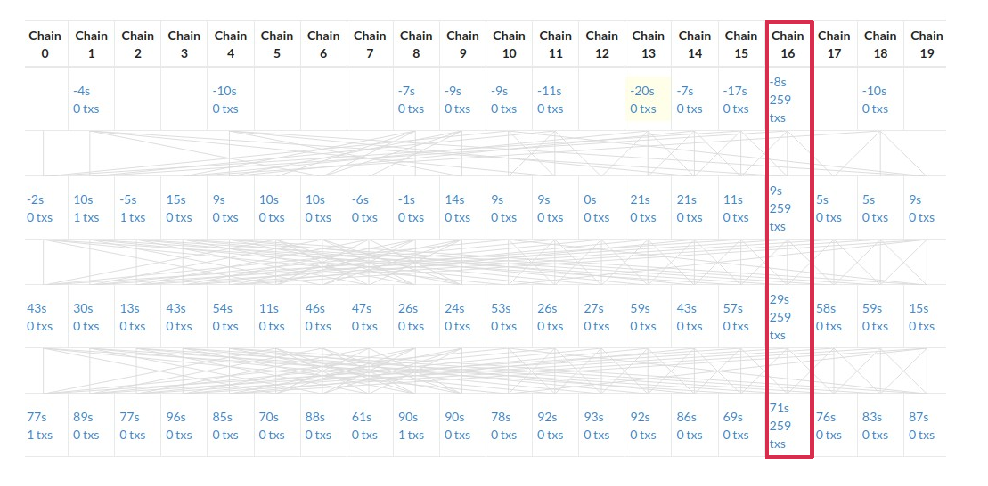
\includegraphics[width=1\linewidth]{images/explorer_crop.pdf}
	\caption{Visuelle Darstellung der Ketten. \cite{KadenaLCC.}} 
	\label{fig:explorer_chain16_result}
\end{figure}

\subsection{Bestimmung des Durchflusses mehrerer Ketten}
Bei dem im Kapitel \eqref{sec:durchfluss_kette} dargestellten Versuch wurde eine Kette verwendet. Doch das Chainweb besteht aus beliebig vielen Ketten $C$. Folglich kann die Anzahl der Transaktionen pro Sekunde durch $TPS_C = C \cdot M$ berechnet werden. Grafik \eqref{fig:tps_chain} stellt den Sachverhalt visuell dar.

\begin{figure}[h!]
    \begin{tikzpicture}
      \begin{axis}[ 
        xlabel=$Ketten \ C$,
        ylabel={$TPS$}
      ] 
        \addplot[domain=0:5000] {x*8}; 
      \end{axis}
    \end{tikzpicture}
\caption{Darstellung des Durchflusses in Abhängigkeit der Ketten.}
\label{fig:tps_chain}
\end{figure}

Man kann erkennen, dass der Durchfluss beim Hinzufügen neuer Ketten linear steigt.

\subsection{Skalierung einer POW-Blockchain durch das Chainweb}
Nun stellt sich die Frage, ob es ein Limit für die Anzahl der Ketten $C$ gibt. Ausschlaggebend dafür sind Grad und Durchmesser des Graphen. In Abbildung \eqref{fig:petersen_graph_10} wurde ein Graph dritten Grades mit dem Durchmesser 2 vorgestellt. Tabelle \eqref{tab:graphentheory} zeigt die mögliche Ordnung eines bekannten Graphen in Abhängigkeit seines Durchmessers $k$ und Grades $d$. 
Es fällt auf, dass mit steigendem Durchmesser und höherem Grad die Ordnung des Graphen steigt. Unter Berücksichtigung der Blockzeit von 30 Sekunden ist ein geringer Durchmesser wünschenswert, da das in Kapitel \eqref{sec:chainweb_overview} beschriebene Simple Payment Verification Protokoll pro Kette eine Blockzeit zur Verifikation benötigt.

Mit $k = 7$ und $d = 7$ wird eine Ordnung von 52 768 erreicht. Übertragen auf das Chainweb entspricht das mit dem zuvor experimentell bestimmten Durchfluss für eine Kette von $TPS_{1} = 8$ für 52 768 Ketten $TPS_{52768} = 52768 \cdot 8 = 422 144$ Transaktionen pro Sekunde. Dieser Wert ist wesentlich höher als bei klassischen Proof of Work Blockchains.

% https://tex.stackexchange.com/questions/89166/centering-in-tabularx-and-x-columns %
\newcolumntype{Y}{>{\centering\arraybackslash}X}
\begin{table*}[t] % top
    \begin{tabularx}{\textwidth}{|c|c|c|c|c|Y|Y|Y|Y|Y|Y|Y|}
        \hline
        \diagbox{d}{k} & 2 & 3 & 4 & 5 & 6 & 7 & 8 & 9 & 10 \\
        \hline
        3 & 10 & 20 & 38 & 70 & 132 & 196 & 360 & 600 & 1 250 \\
        \hline
        4 & 15 & 41 & 98 & 364 & 740 & 1 320 & 3 243 & 7 575 & 17 703 \\
        \hline
        5 & 24 & 72 & 212 & 624 & 2 772 & 5 516 & 17 030 & 57 840 & 187 056 \\
        \hline
        6 & 32 & 111 & 390 & 1 404 & 7 917 & 19 383 & 76 461 & 331 387 & 1 253 615 \\
        \hline
        7 & 50 & 168 & 672 & 2 756 & 11 988 & 52 768 & 249 660 & 1 223 050 & 6 007 230 \\
        \hline
        8 & 57 & 253 & 1 100 & 5 060 & 39 672 & 12 127 & 734 820 & 4 243 100 & 24 897 161 \\
        \hline
        9 & 74 & 585 & 1 550 & 8 268 & 75 893 & 279 616 & 1 697 688 & 12 123 288 & 65 866 350 \\
        \hline
        10 & 91 & 650 & 2 286 & 13 140 & 134 690 & 583 083 & 4 293 452 & 27 997 102 & 600 380 000 \\
        \hline
        11 & 104 & 715 & 3 200 & 19 500 & 156 864 & 1 001 268 & 7 442 328 & 72 933 102 & 600 380 000 \\
        \hline
        12 & 133 & 786 & 4 680 & 29 470 & 359 772 & 1 999 500 & 15 924 326 & 158 158 875 & 1 506 252 500 \\
        \hline
        13 & 162 & 851 & 6 560 & 40 260 & 531 440 & 3 322 080 & 29 927 790 & 249 155 760 & 3 077 200 700 \\
        \hline
        14 & 183 & 916 & 8 200 & 578 37 & 816 294 & 6 200 460 & 55 913 932 & 600 123 780 & 7 041 746 081 \\
        \hline
        15 & 187 & 1 215 & 11 712 & 76 518 & 1 417 248 & 8 599 986 & 90 001 236 & 1 171 998 164 & 10 012 349 898 \\
        \hline
        16 & 200 & 1 600 & 14 640 & 132 496 & 1 771 560 & 14 882 658 & 140 559 416 & 2 025 125 476 & 12 951 451 931 \\
        \hline
    \end{tabularx}
\caption{Ordnung eines Graphen mit Grad $d$ und Durchmesser $k$. \cite{Beardsley.2021}}
\label{tab:graphentheory}
\end{table*}